\subsection{Klassediagram}
For at illustrere modellaget i vores MVC-mønster, har vi produceret et klassediagram (se \myref{diagram:klassediagram} nedenfor) i UML, der simplificerer strukturen.

\begin{figure}[H]
\centering
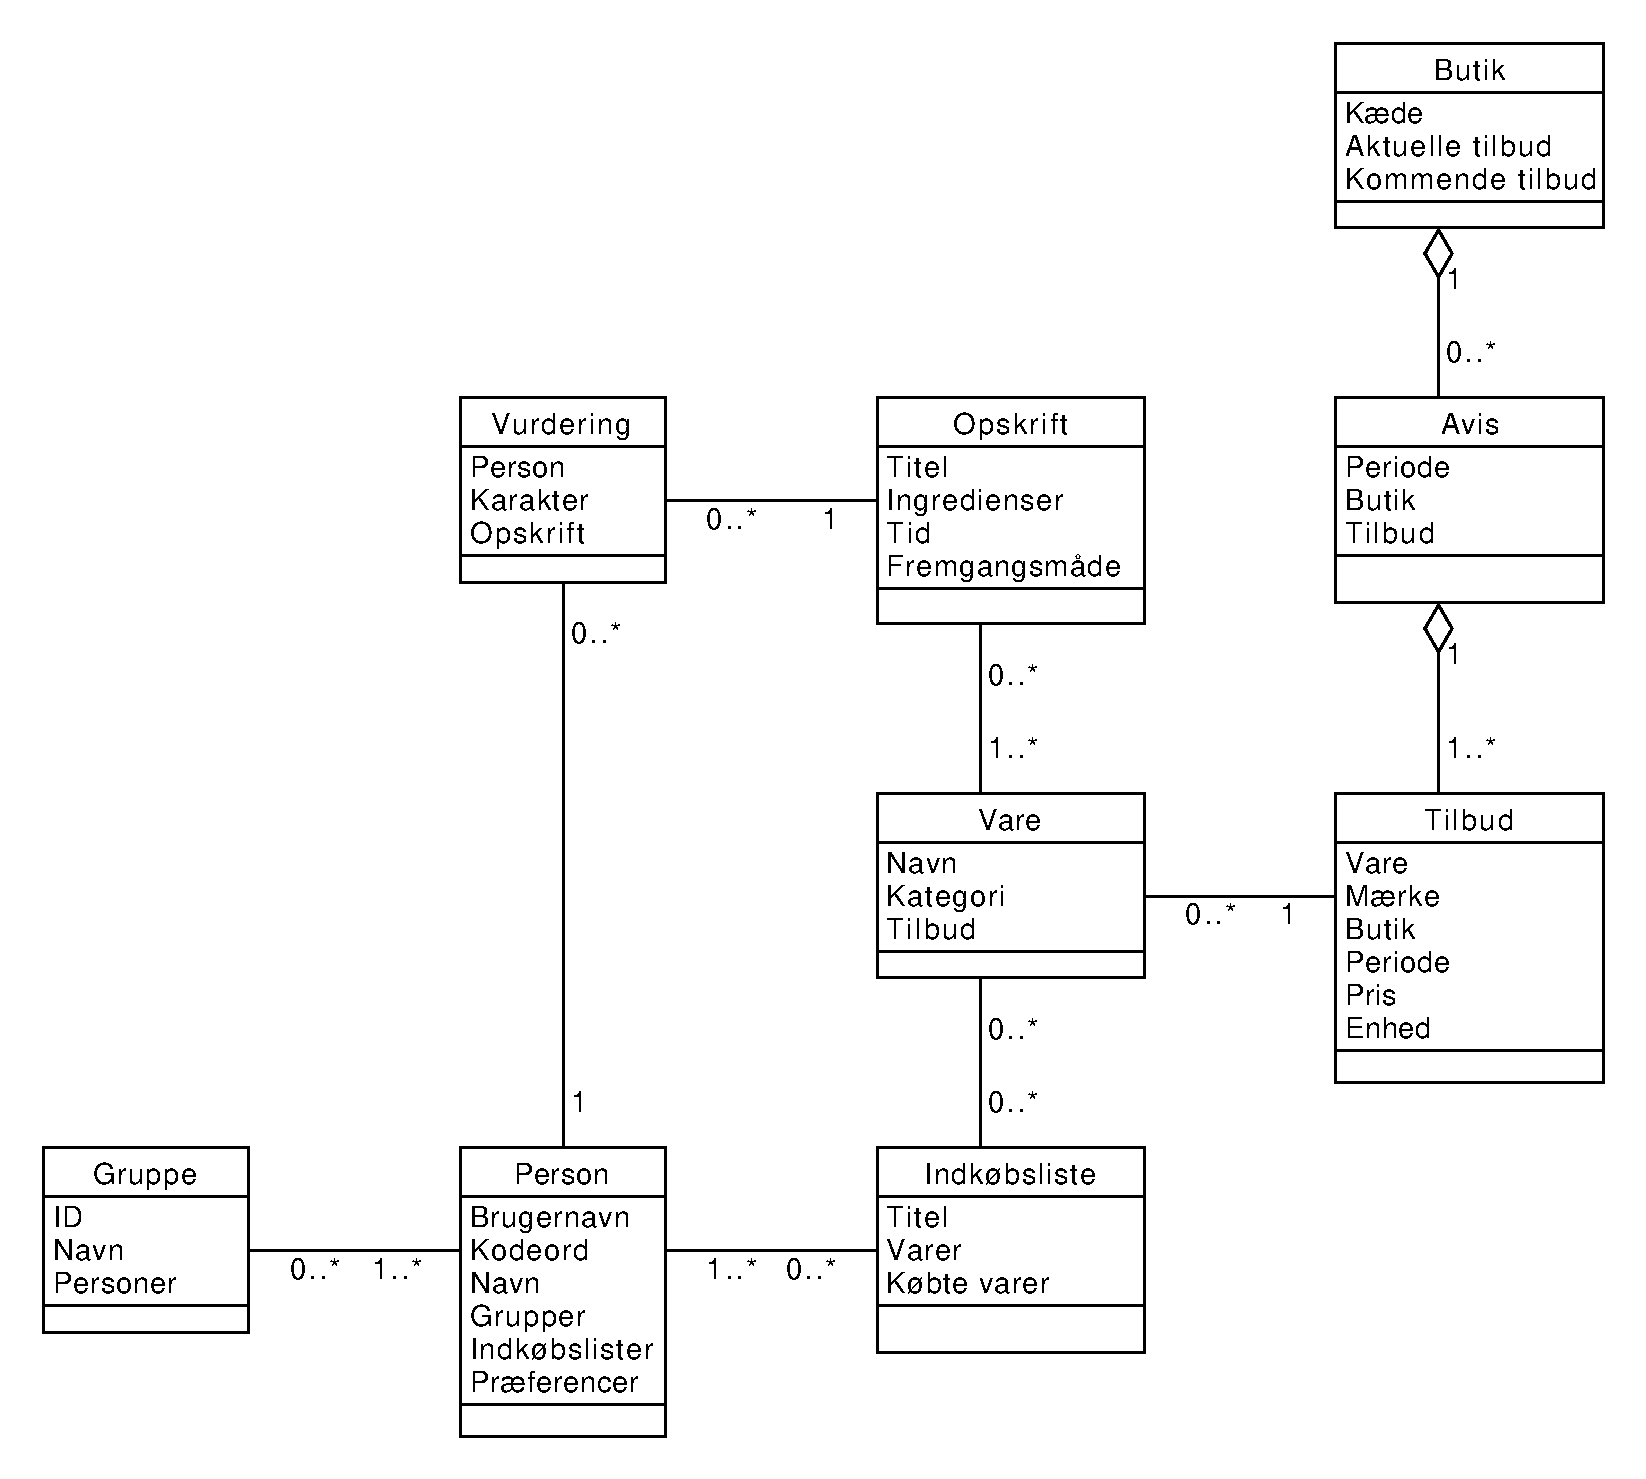
\includegraphics[width=0.8\linewidth]{/Diagrams/klassediagram_model_expanded_implemented.pdf}
\caption{UML klassediagram for modellaget i MVC-mønsteret}\label{diagram:klassediagram}
\end{figure}

Der er mange relationer mellem klasserne, da de forskellige klasse indeholder lister af hinanden.
En ShoppingList har en liste over Items, og disse Items har en liste over Offers, for at binde Offer'sne til det pågældende Item.
Recipe har en liste over Items, som bruges som ingredienser.
På denne måde kan de tilføjes til ShoppingList gennem RecipesController, uden at skulle lave nye objekter, som ShoppingList kan læse.
User har en liste over ShoppingLists, samt en liste over Prefs, eller præferencer, for at gøre hjemmesiden mere personlig og fokuseret på brugeren som er logget ind.
Der er relationstabeller mellem many-to-many forholdene, som gør det muligt at gemme ekstra værdier ved et af forholdene.
F.eks. når man tilføjer et Item til en ShoppingList eller en Recipe, kan man angive mængder af disse Items.
Dette gøres igennem relationsklasserne, Recipe\textunderscore Ingredient, og ShoppingList\textunderscore item.

I de følgende afsnit, vil der gives en gennemgang af udvalgte dele af komponenterne fra \myref{subsec:komp}.
